\section{Problema 3}
\begin{tcolorbox}[colback=gray!15,colframe=gray!1!gray,title=Teorema caracterización monótono (demostrado en clase)]
	Suponga que $f:(a, b) \rightarrow \mathbb{R}$ es diferenciable sobre $(a, b)$. Entonces,\newline
	(1) $f$ es creciente ssi $f^{\prime}(x) \geqslant 0$, $\quad  \forall x \in(a, b)$.\newline
	(2) $f$ es decreciente ssi $f^{\prime}(x) \leqslant 0, \quad \forall x \in(a, b)$
\end{tcolorbox}
\begin{noter}{Teorema importante}
	Para resolver los siguientes problemas que se presentan, primero se demostrará \textit{con un método alternativo} el siguiente teorema de \cite{bartle2000introduction}. 
	\begin{tcolorbox}[colback=gray!15,colframe=gray!1!gray,title=Teorema  6.4.6]
		Let $I$ be an open interval and let $f : I \to \mathbb{R}$ have a second derivative on $I$. Then $f$ is a convex function on $I$ if and only if $f''(x)\geq 0$ for all $x \in I$.
	\end{tcolorbox}


\begin{proof}
	Es un teorema de caracterización, por lo cual: 
	\begin{enumerate}
		\item $(\to)$ Trivial. Por el teorema resuelto en el \textbf{Problema 1}, sabemos que $f'$ es creciente. Ahora bien, por el teorema de caracterización monótono (demostrado en clase) sabemos que $f''(x)\geq 0$. 
		\item $(\gets)$ Se tomará en cuenta la idea de \cite{tiel1984convex}. 
		Sea $x, y \in I, x<y$ y $\lambda\in (0,1)$. Por \textbf{teorema del valor medio} de \cite{bartle2000introduction}, sabemos que existe\newline $$\xi_{1}, \xi_{2}, x<\xi_{1}<\lambda x+(1-\lambda) y<\xi_{2}<y$$y  $$\xi_{3}, \xi_{1}<\xi_{3}<\xi_{2}$$
		tal que
		$$
		\begin{aligned}
			f(\lambda&x+(1-\lambda) y)-\lambda f(x)-(1-\lambda) f(y) \\
			&=\lambda[f(\lambda x+(1-\lambda) y)-f(x)]+(1-\lambda)[f(\lambda x+(1-\lambda) y)-f(y)] \\
			&=\lambda(1-\lambda)(y-x) f^{\prime}\left(\xi_{1}\right)+(1-\lambda) \lambda(x-y) f^{\prime}\left(\xi_{2}\right) \\
			&=\lambda(1-\lambda)(y-x)\left(\xi_{1}-\xi_{2}\right) f^{\prime \prime}\left(\xi_{3}\right) \leqslant 0 .
		\end{aligned}
		$$
		Por lo tanto $f$ es convexo.
	\end{enumerate}
\end{proof}
\end{noter}
Compruebe que la función: 
\begin{enumerate}
	\item $f(x)=e^x$ es convexa. 
	\begin{figure}[ht]
		\centering
		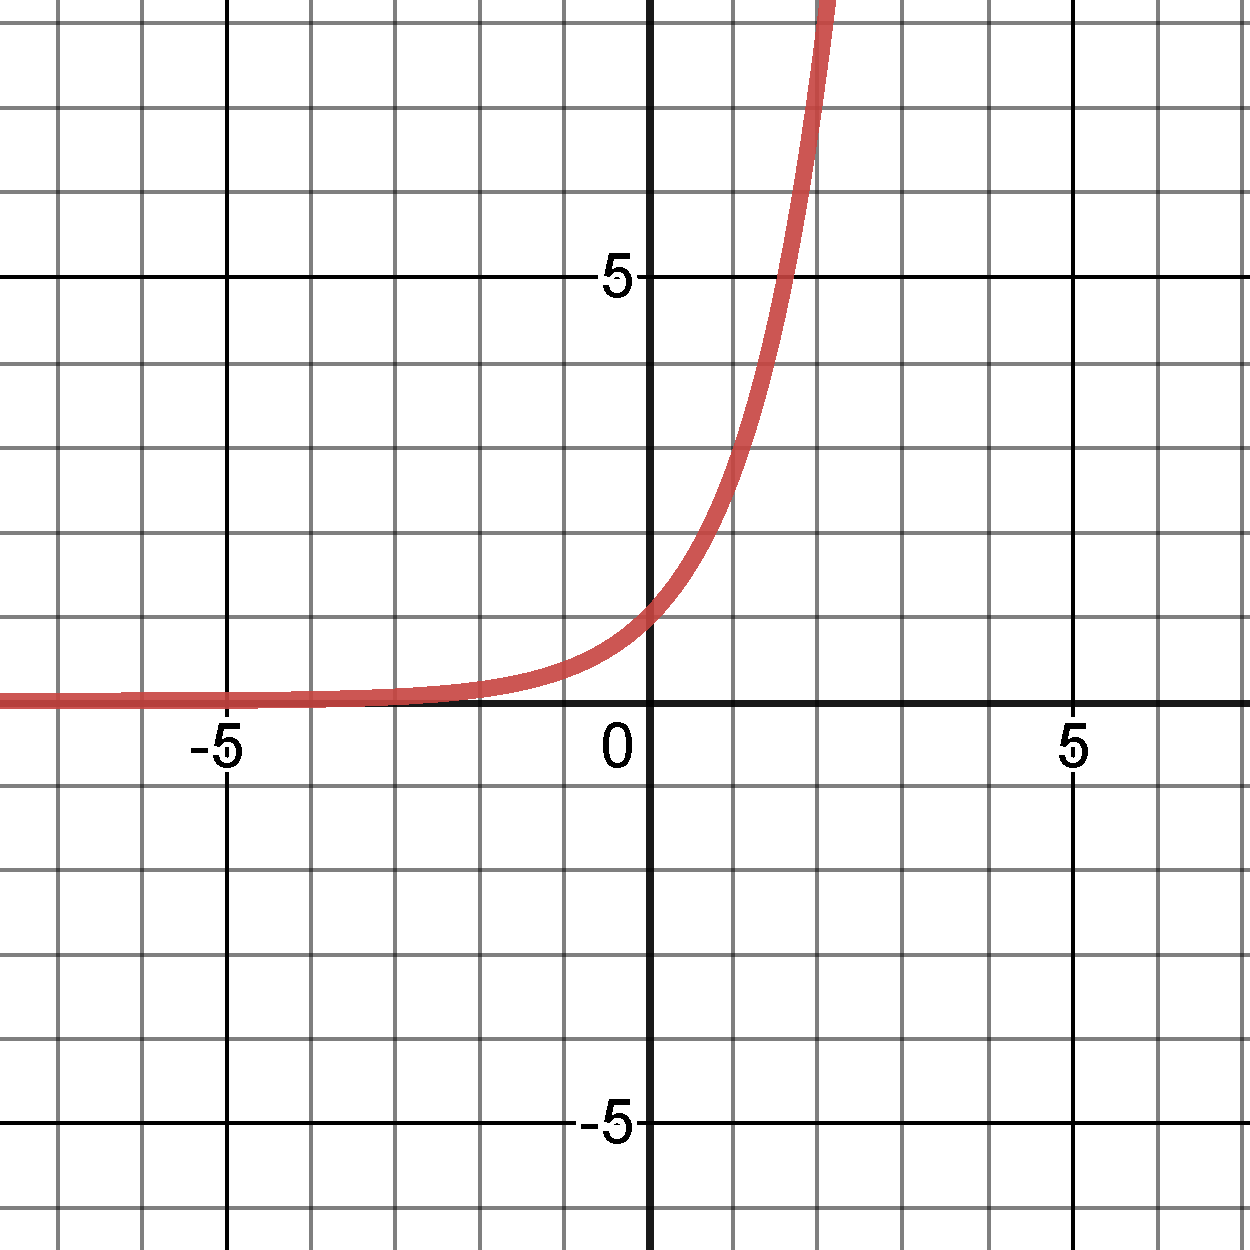
\includegraphics[scale=0.3]{/Users/rudiks/Git/Real_Analysis/HT5/Imagenes/1.pdf}
		\caption{$f(x)=e^x$}
	\end{figure}

		\begin{proof}
		Por el \textbf{teorema importante}, entonces se tiene: 
		$$\implies f(x)=e^x \implies f'(x) =e^x \implies f''(x)= e^x.$$
		Entonces, $f''(x)\geq 0$. Por lo tanto, es una función convexa.
	\end{proof}


%--------------------------

	\item $f(x)=\ln x$ es cóncava. 
		\begin{figure}[ht]
		\centering
		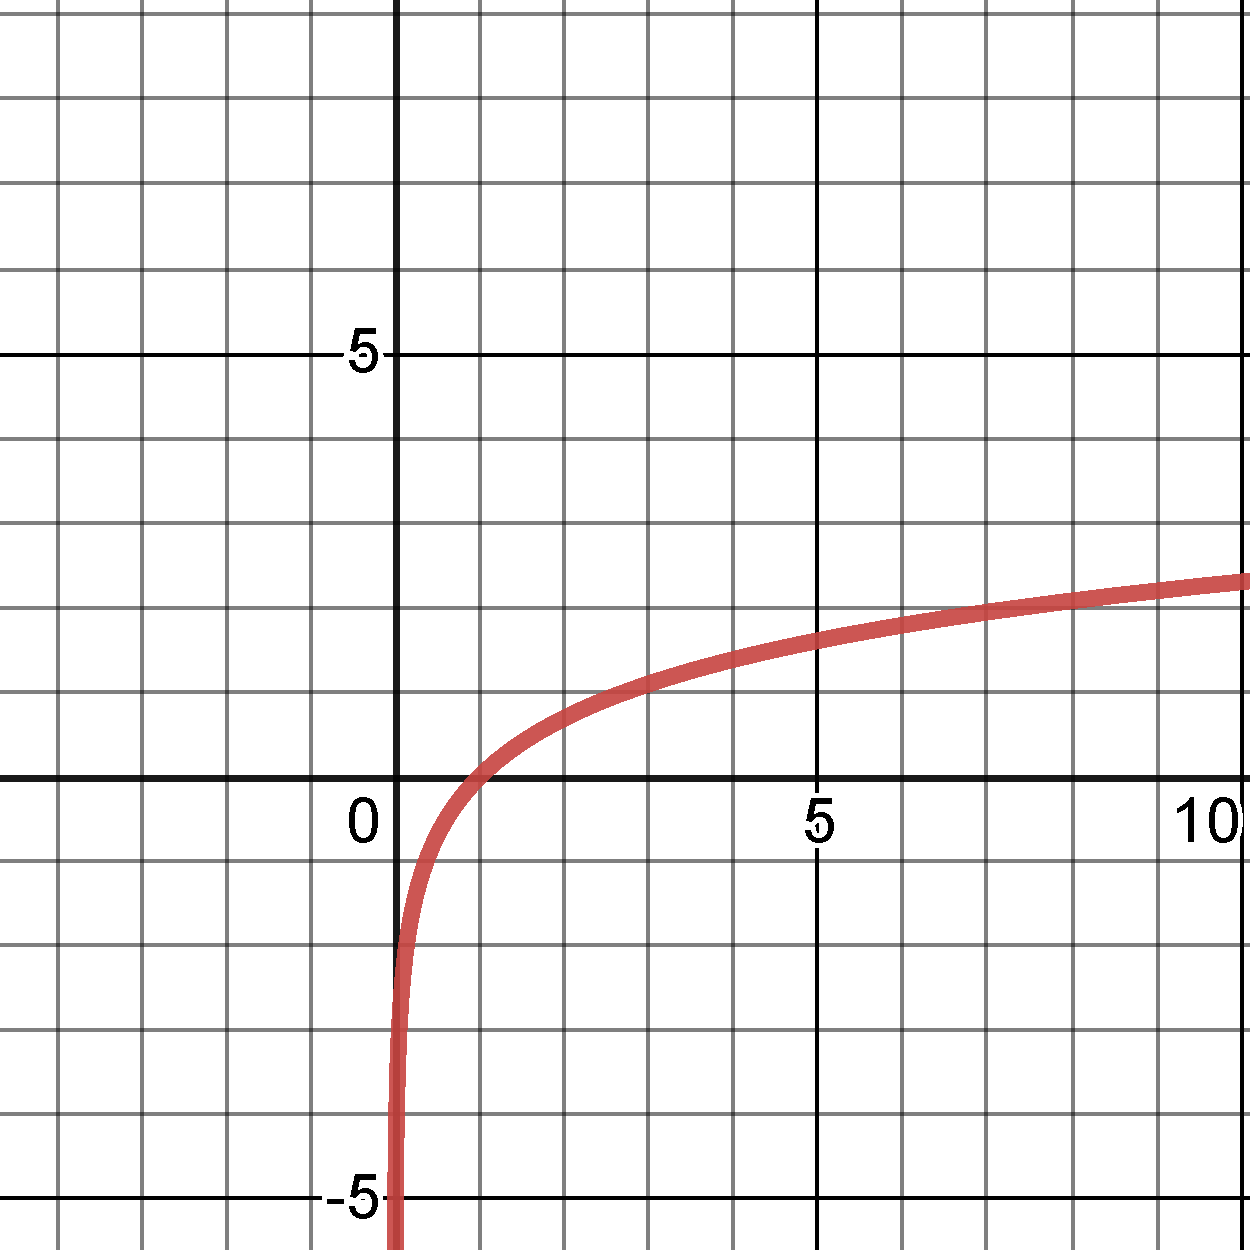
\includegraphics[scale=0.3]{/Users/rudiks/Git/Real_Analysis/HT5/Imagenes/2.pdf}
		\caption{$f(x)=\ln x$}
	\end{figure}
		\begin{proof}
		Por la definición de cóncavo, se probará: $f(x)=-\ln x$ es convexa. Por el \textbf{teorema importante}:
		$$\implies f(x)=-\ln x\implies f'(x)=-\frac{1}{x}\implies f''(x)=\frac{1}{x^2}.$$
		Entonces, $f''(x)\geq 0$. Por lo tanto, es una función convexa. Por la definición, entonces $f(x)=\ln x$ es cóncava. 
	\end{proof}


%--------------------------





	\item $f(x)=x^\alpha$, es $\begin{cases}
		\text{Convexa, si} & \alpha \leq 0 \text{ o } \alpha \geq 1\\
		\text{Cóncava, si} & 0 \leq \alpha \leq 1
	\end{cases}$
\begin{figure}[ht]
	\begin{tabular}{cc}
		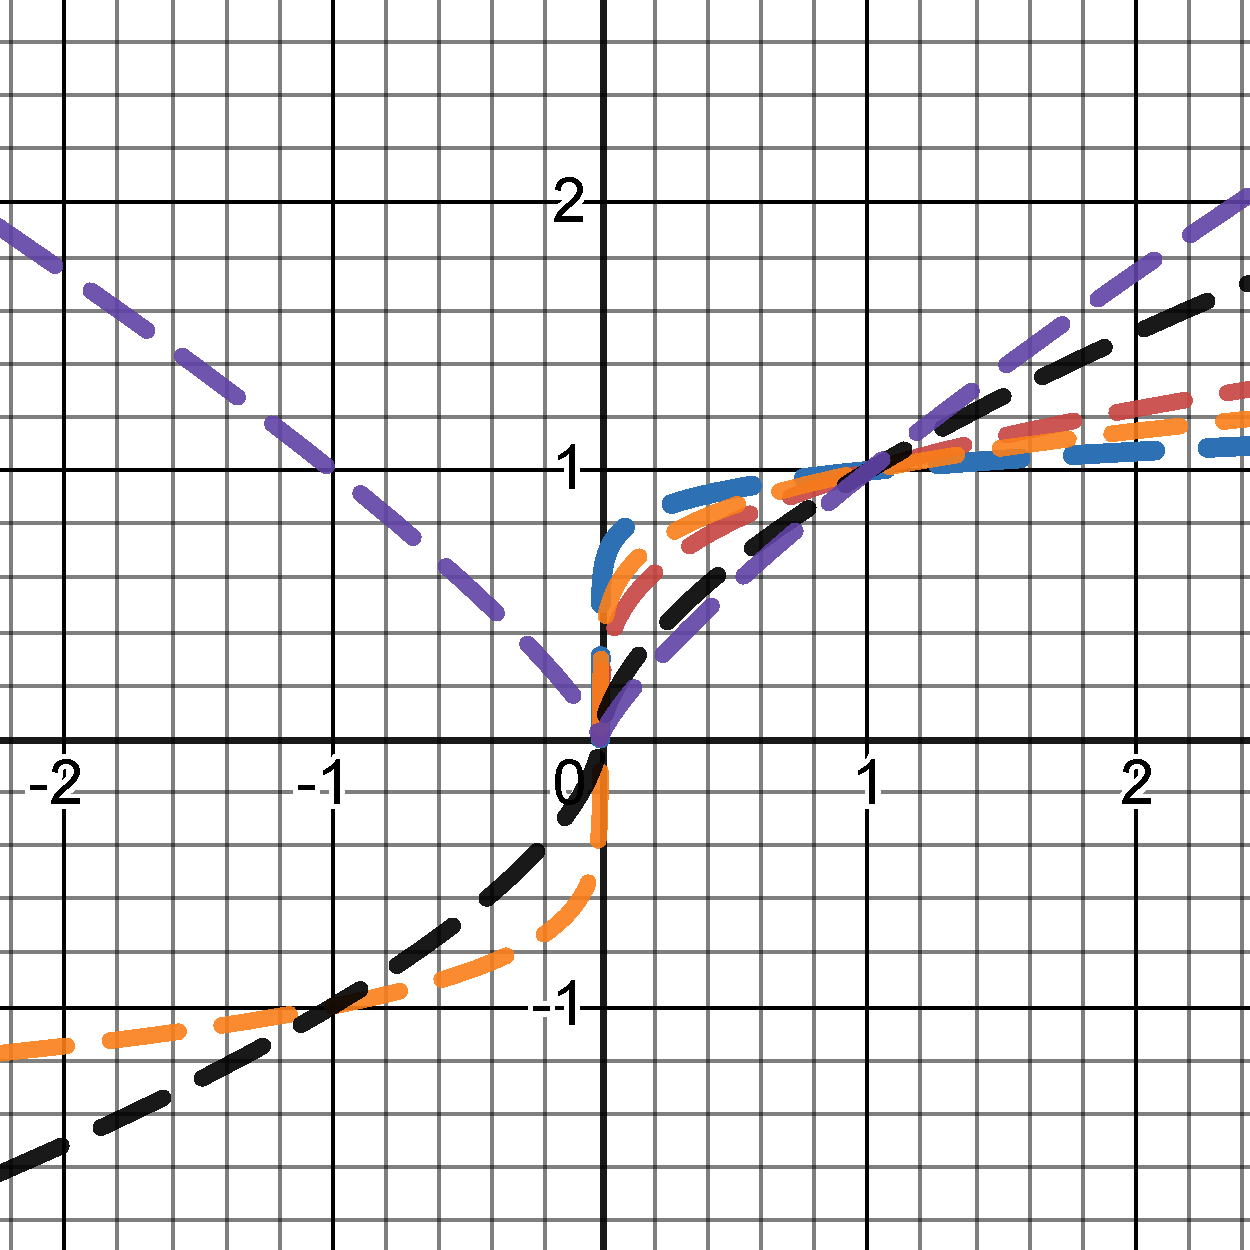
\includegraphics[width=65mm]{/Users/rudiks/Git/Real_Analysis/HT5/Imagenes/3.1.pdf} &   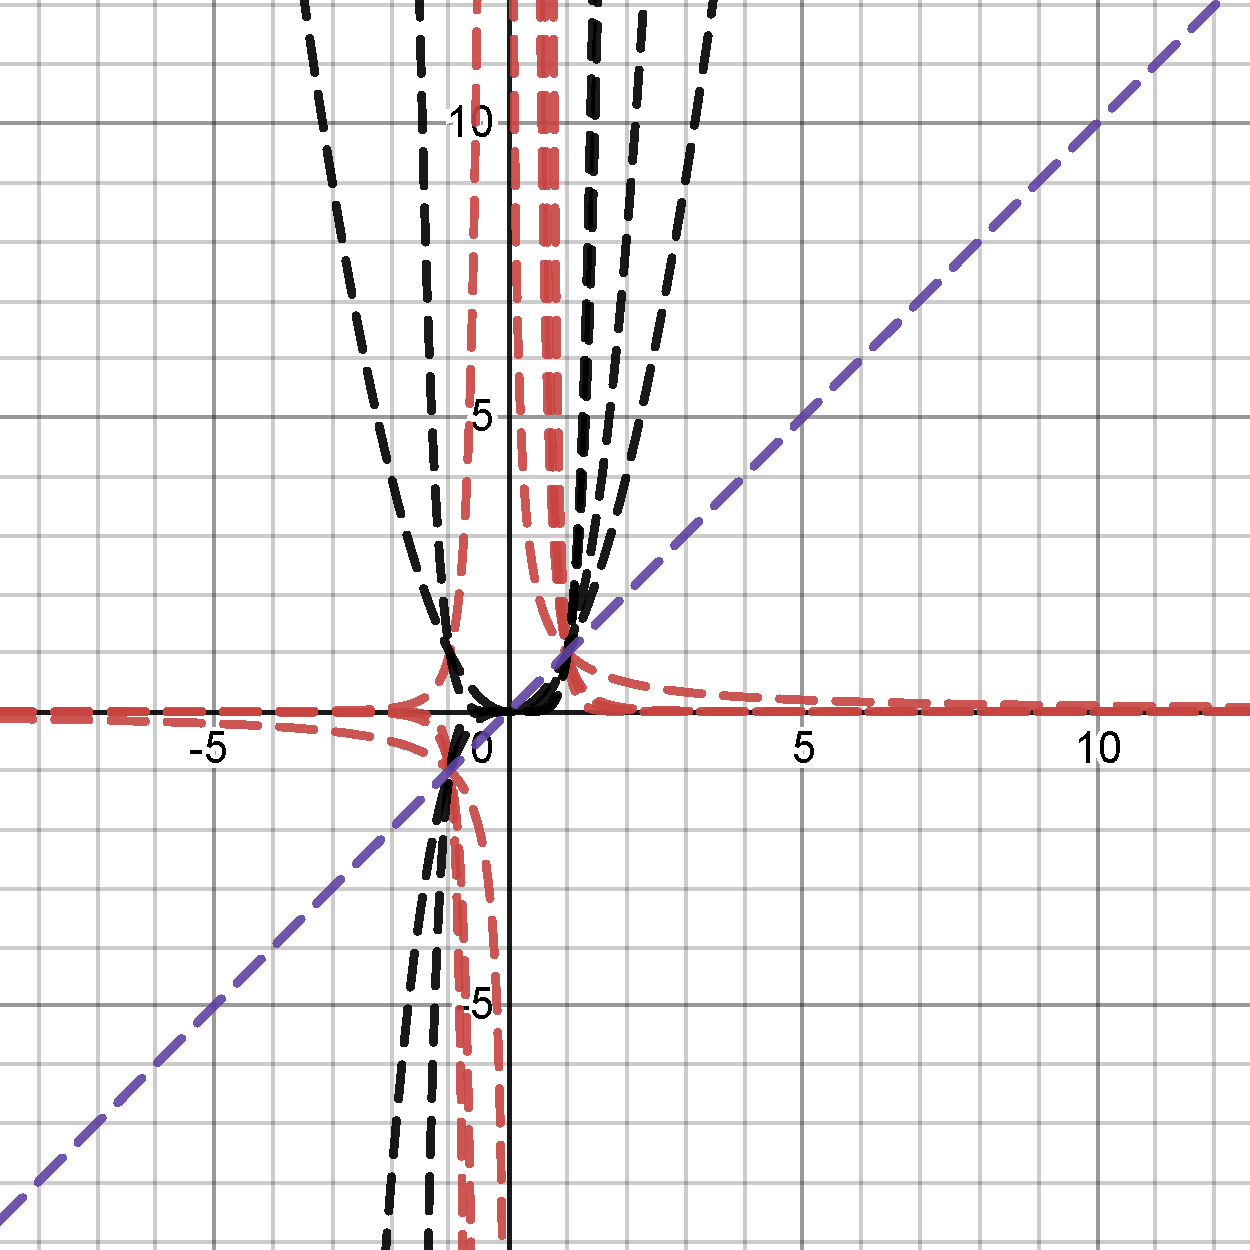
\includegraphics[width=65mm]{/Users/rudiks/Git/Real_Analysis/HT5/Imagenes/3.2.pdf} \\
		(a) $\alpha \leq 0 \text{ o } \alpha \geq 1$ & (b) $0 \leq \alpha \leq 1$
	\end{tabular}
	\caption{$f(x)=x^\alpha$}
\end{figure}
	\begin{proof}Comenzamos calculando la segunda derivada: 
		\begin{gather}
			\implies f(x)=x^\alpha \implies f'(x)=\alpha x^{\alpha -1}\implies f''(x)=\alpha (\alpha -1)x^{\alpha -2}.
		\end{gather}
	Análogamente: 
	\begin{gather}
		\implies f(x)=-x^\alpha \implies f'(x)=-\alpha x^{\alpha -1}\implies f''(x)=-\alpha (\alpha -1)x^{\alpha -2}.
	\end{gather}
	Nótese que tenemos dos casos:
	\begin{enumerate}
		\item $f(x)=x^\alpha$ es convexa, $\alpha \leq 0$ o $\alpha \geq 1$. Es decir, tenemos: $$\alpha \in (-\infty, 0] \qquad \text{ o }\qquad  \alpha \in [1,\infty).$$
		Considérese la segunda derivada obtenida en (1), por el \textbf{teorema importante} la condición se cumple trivialmente para $\alpha \in (-\infty,0]\cup [1,\infty)$; ya que $f''(x)\geq 0$ en todos los casos. Por lo tanto es convexa.
		\item $f(x)=x^\alpha$ es cóncava, $0\leq \alpha \leq 1$. Es decir, tenemos:
		$$a\in [0,1].$$
			Por la definición de cóncavo, se probará $x^\alpha$ es convexa. Considérese la segunda derivada de $f(x)=-x^{\alpha}$ obtenida en (3), por el \textbf{teorema importante} la condición se cumple trivialmente para $\alpha \in [0,1]$; ya que $f''(x)\geq 0$ en todos los casos. Por lo tanto es convexa y por la definición de función cóncava, $x^\alpha$ es cóncava en $a\in [0,1]$.
	\end{enumerate}
\end{proof}
\end{enumerate}